\section{Problem 3}
\textit{Assuming a DVB-H system enhanced with short range communication technologies similar to the one studied in class but nodes attempting to watch one channel. Assume the transmit and receive power for short range communication is Ptsr and Prsr, respectively, and that the receive power from the cellular base station is Prc. Assume that n receivers are part of a cooperative cluster and that the loss probability of packets coming from the cellular base station and from other nodes in the cluster is ec and ed, respectively. Calculate the mean energy consumption for the following scenarios.}

\subsection{a)}
\textit{Nodes in the cooperative cluster nominate a cluster head that overhears transmissions from the base station and exchange packets to the others using unicast transmissions that rely on an ARQ mechanism.}\\
The way the system works is illustrated in figure \ref{fig1:MM11_ex3}, where n number of nodes is existing in the cluster and node n = 1 is the cluster head.
\begin{figure}[!h]
  \centering
  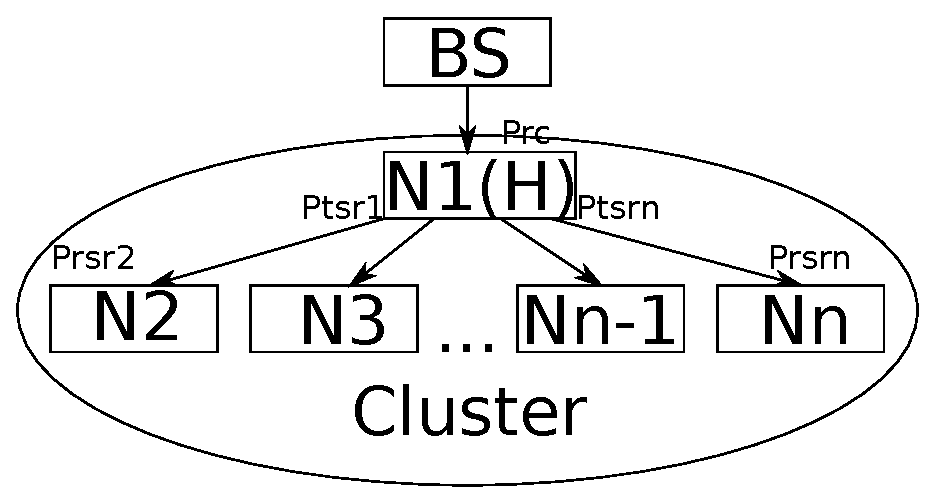
\includegraphics[width=6cm]{mm11_exc_3_1.eps}
  \caption{Cooperative cluster with cluster head distributing the packets}
  \label{fig1:MM11_ex3}
\end{figure}


To calculate the energy the power needs to be related to time. So for transmission from base station to nodes the energy used is $E_{rc} = P_{rc} \cdot t_{1}$ and between the nodes $E_{rsr} = P_{rsr} \cdot t_{2}$ given the time for transmitting the data and receiving it is the same the energy for transmission is $E_{tsr} = P_{tsr} \cdot t_{2}$. The energy used for the cluster head to receive the packet is $E_{rch} = \frac{E_{rc}}{ec}$. The energy used for the cluster head to transmit to the rest of the clusters and for those to receive it using unicast is $E_{chc} = (n-1) \cdot \frac{(E_{tsr} + E_{rsr})}{ed}$. The total energy used to transmit the data from the base station to the cluster is 
\begin{flalign}
 && E_{total}=& E_{rch} + E_{chc}& \\
 && =& \frac{E_{rc}}{ec} +  (n-1) \cdot \frac{(E_{tsr} + E_{rsr})}{ed}&
\end{flalign}



\subsection{b)}
\textit{Nodes in the cooperative cluster receive directly from the base station.}\\
The way the system works is illustrated in figure \ref{fig2:MM11_ex3}, where n number of nodes is existing in the cluster.
\begin{figure}[!h]
  \centering
  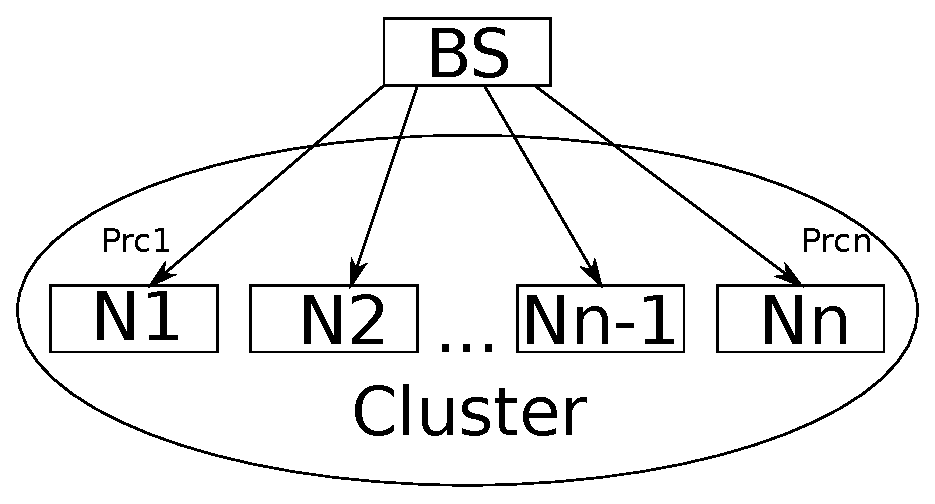
\includegraphics[width=6cm]{mm11_exc_3_2.eps}
  \caption{Cooperative cluster with the base station distributing the packets}
  \label{fig2:MM11_ex3}
\end{figure}
Same assumptions applies as in \textbf{a)} but here all nodes receives from the base station. So the energy used to transmit to all is 
\begin{flalign}
 && E_{total}=&n \cdot \frac{P_{rc} \cdot t}{ec} &
\end{flalign}


Depending on how the parameters are for the two cases one can prove to be better than the other. If the short range communication is using much less power than the long range (BS). Either the time it takes to transmit or the probability of error can be higher. This can off cause also work the other way around so depending on the two technologies one both cases can be the preferred.  